\chapter{论文构成}
毕业论文(设计)是培养学生综合运用本学科的基本理论、专业知识和基本技能,提高分析和解决实际问题的能力,完成初步培养从事科学研究工作和专业工程技术工作基本训练的重要环节。为了统一和规范我校本科生毕业论文(设计)的写作,保证我校本科生毕业论文(设计)的质量,根据《中华人民共和国国家标准学位论文编写规则》(国家标准GBT7713.1-2006)的规定特制定《湖南大学本科生毕业论文(设计)撰写规范(大理类)》:
xxxxxxxxxxx

毕业论文(设计)是培养学生综合运用本学科的基本理论、专业知识和基本技能,提高分析和解决实际问题的能力,完成初步培养从事科学研究工作和专业工程技术工作基本训练的重要环节。为了统一和规范我校本科生毕业论文(设计)的写作,保证我校本科生毕业论文(设计)的质量,根据《中华人民共和国国家标准学位论文编写规则》(国家标准GBT7713.1-2006)的规定特制定《湖南大学本科生毕业论文(设计)撰写规范(大理类)》:
xxxxxxxxxxx

毕业论文(设计)是培养学生综合运用本学科的基本理论、专业知识和基本技能,提高分析和解决实际问题的能力,完成初步培养从事科学研究工作和专业工程技术工作基本训练的重要环节。为了统一和规范我校本科生毕业论文(设计)的写作,保证我校本科生毕业论文(设计)的质量,根据《中华人民共和国国家标准学位论文编写规则》(国家标准GBT7713.1-2006)的规定特制定《湖南大学本科生毕业论文(设计)撰写规范(大理类)》:
xxxxxxxxxxx

毕业论文(设计)是培养学生综合运用本学科的基本理论、专业知识和基本技能,提高分析和解决实际问题的能力,完成初步培养从事科学研究工作和专业工程技术工作基本训练的重要环节。为了统一和规范我校本科生毕业论文(设计)的写作,保证我校本科生毕业论文(设计)的质量,根据《中华人民共和国国家标准学位论文编写规则》(国家标准GBT7713.1-2006)的规定特制定《湖南大学本科生毕业论文(设计)撰写规范(大理类)》:
xxxxxxxxxxx

毕业论文(设计)是培养学生综合运用本学科的基本理论、专业知识和基本技能,提高分析和解决实际问题的能力,完成初步培养从事科学研究工作和专业工程技术工作基本训练的重要环节。为了统一和规范我校本科生毕业论文(设计)的写作,保证我校本科生毕业论文(设计)的质量,根据《中华人民共和国国家标准学位论文编写规则》(国家标准GBT7713.1-2006)的规定特制定《湖南大学本科生毕业论文(设计)撰写规范(大理类)》:
xxxxxxxxxxx

学位论文包括前置部分、正文部分、附录部分、附件。具体构成如图\ref{fig:struct}:
\begin{figure}
\centering
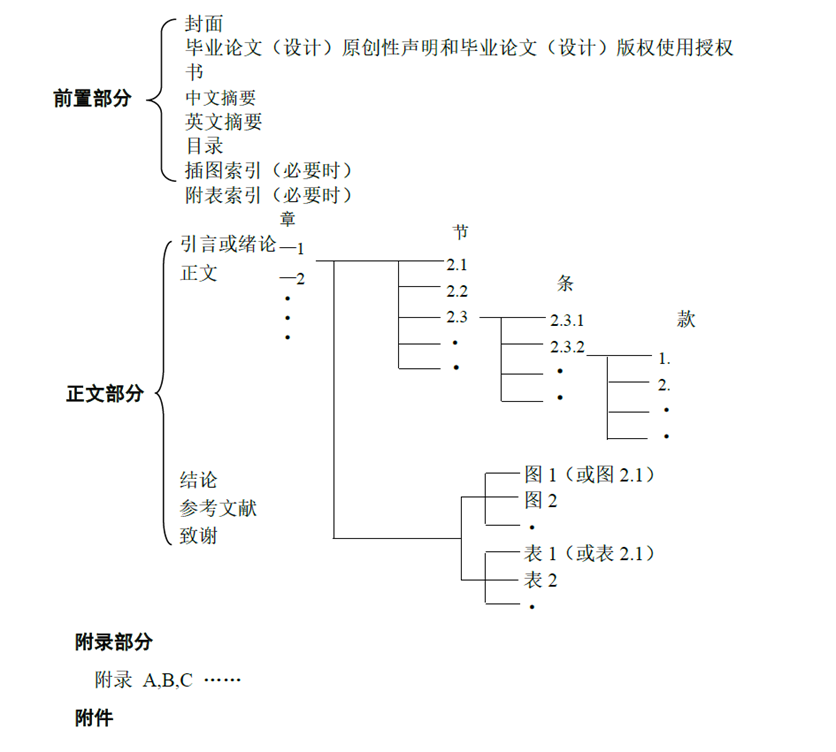
\includegraphics[width=0.9\linewidth]{docs/imgs/structure}

\vspace{-8pt}
\notes 前置部分、正文部分、附录部分、附件
\vspace{-8pt}
\caption{论文结构与框架}\label{fig:struct}
\end{figure}
